\documentclass[border=10pt]{standalone}

\usepackage{tikz}
\usepackage{tikzsymbols}
\usetikzlibrary{calc,patterns,shapes.geometric}

\def\centerarc[#1](#2)(#3:#4:#5){\draw[#1] ($(#2)+({#5*cos(#3)},{#5*sin(#3)})$) arc (#3:#4:#5);}

\begin{document}
	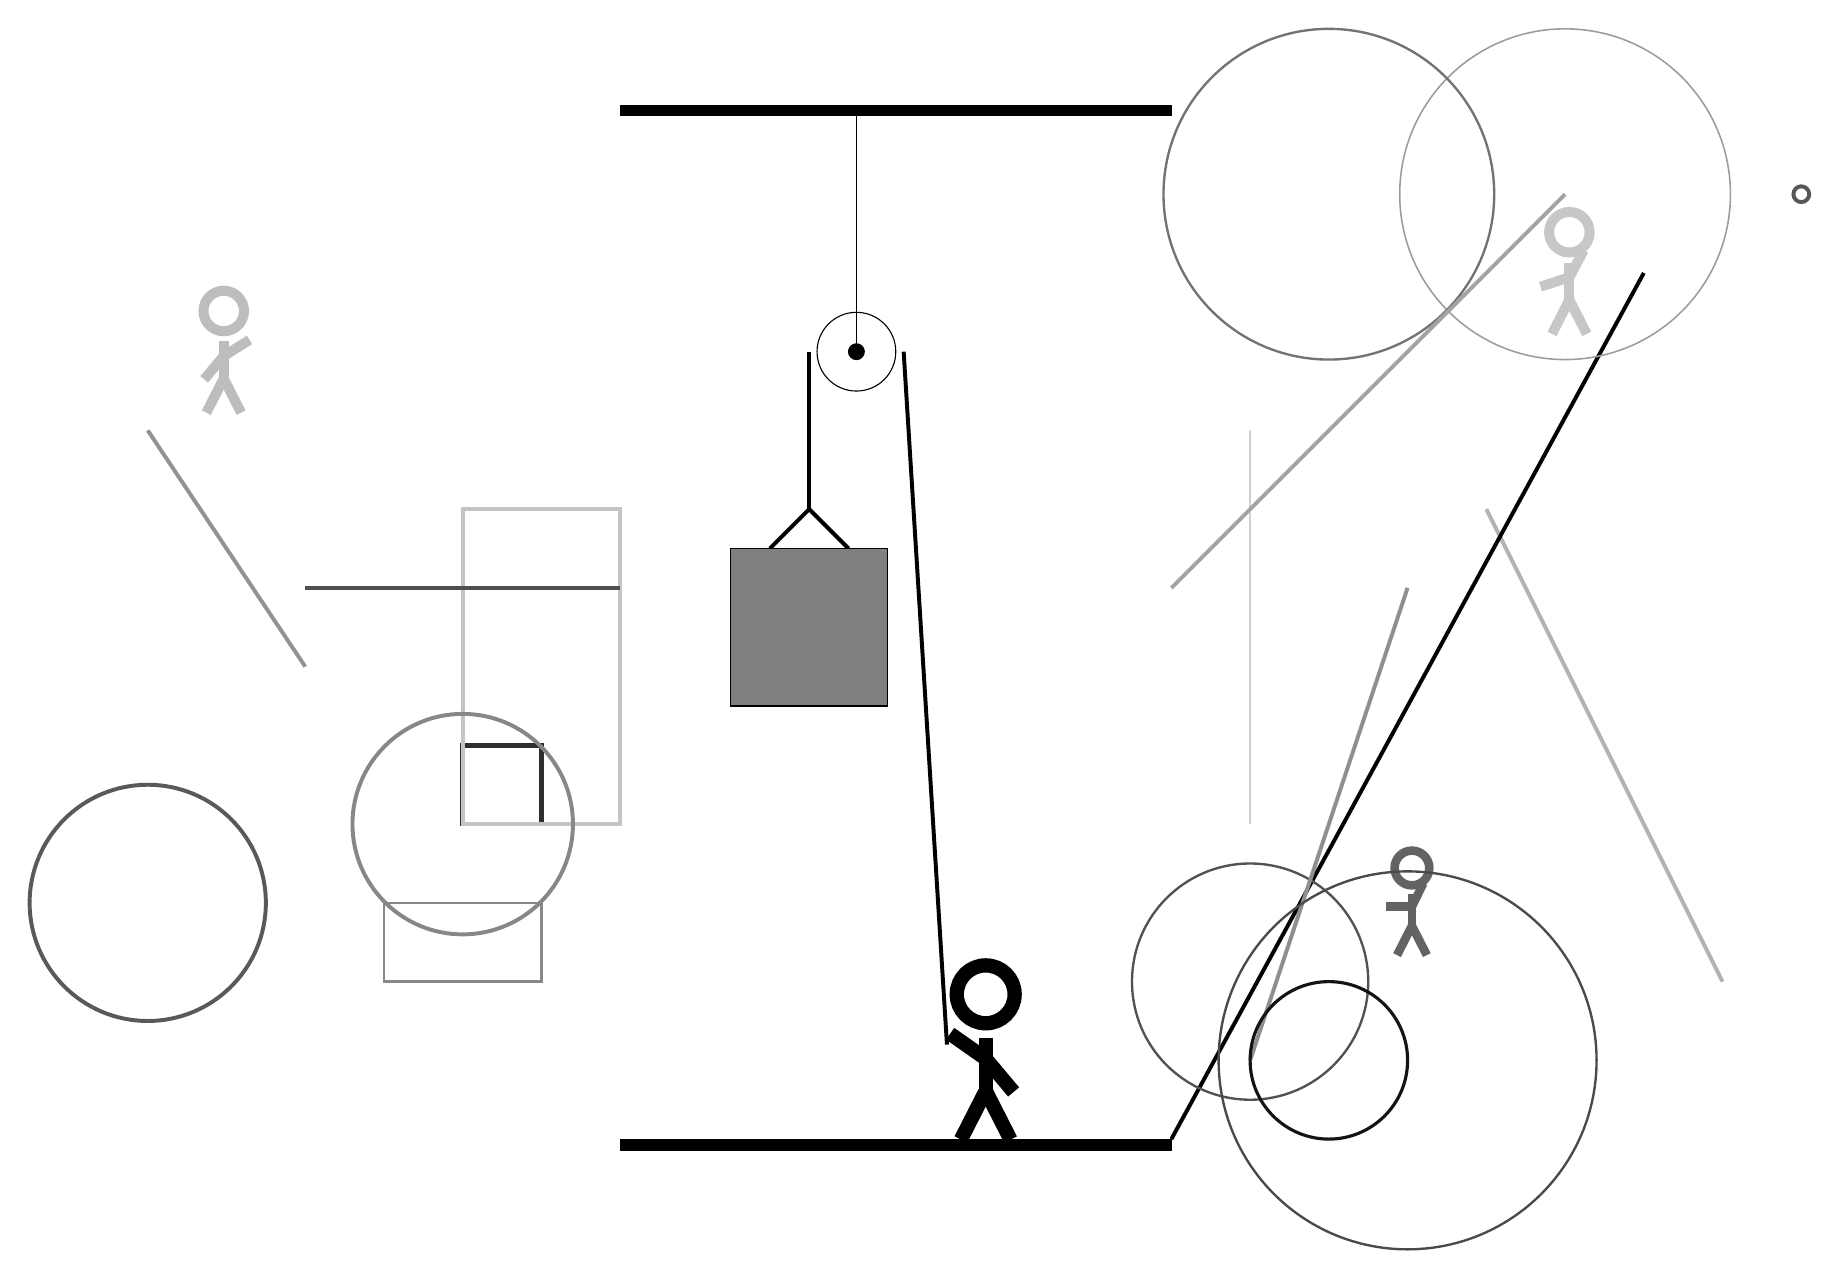
\begin{tikzpicture}
		%%%%% START %%%%%
		
		\draw[fill=black] (-2, 10) rectangle (5, 10.125);
		
		\draw (1, 7) circle (0.5);
		\draw[fill=black] (1, 7) circle (0.1);
		\draw (1, 10) -- (1, 7);
		
		\draw[line width=0.5mm] (-0.1, 4.5) -- (0.4, 5.0) -- (0.9, 4.5);
		\draw[fill=black!50] (-0.6, 4.5) rectangle (1.4, 2.5);
		
		\draw[line width=0.6mm, color=black!82] (-4, 1) rectangle (-3, 2);
		
		\draw[line width=0.5mm, color=black!30](9, 5) -- (12, -1);
		\draw[line width=0.5mm, color=black!99](5, -3) -- (11, 8);
		\draw [line width=0.2mm, color=black!54](8, 3) circle (0.0);
		
		\draw[line width=0.3mm, color=black!47] (-3, -1) rectangle (-5, 0);
		
		\draw [line width=0.5mm, color=black!65](-8, 0) circle (1.5);
		\draw[line width=0.5mm, color=black!43](-6, 3) -- (-8, 6);
		\draw [line width=0.3mm, color=black!68](6, -1) circle (1.5);
		\node[line width=0.7mm, color=black!26] at (-7, 7) {\Strichmaxerl[7][50][32]};
		\draw [line width=0.2mm, color=black!39](10, 9) circle (2.1);
		\draw[line width=0.3mm, color=black!18] (6, 6) rectangle (6, 1);
		
		\draw[line width=0.5mm, color=black!44](6, -2) -- (8, 4);
		\draw [line width=0.4mm, color=black!92](7, -2) circle (1.0);
		
		\draw[line width=0.5mm, color=black!23] (-2, 5) rectangle (-4, 1);
		\draw [line width=0.3mm, color=black!55](7, 9) circle (2.1);
		\draw [line width=0.5mm, color=black!47](-4, 1) circle (1.4);
		\draw[line width=0.5mm, color=black!36](5, 4) -- (10, 9);
		
		\node[line width=0.6mm, color=black!22] at (10, 8) {\Strichmaxerl[7][18][62]};
		\draw[line width=0.5mm, color=black!69](-6, 4) -- (-2, 4);
		
		\node[line width=0.7mm, color=black!61] at (8, 0) {\Strichmaxerl[6][0][64]};
		\draw [line width=0.5mm, color=black!66](13, 9) circle (0.1);
		\draw [line width=0.3mm, color=black!71](8, -2) circle (2.4);
		
		
		\draw[line width=0.5mm] (0.4, 7) -- (0.4, 5.0);
		\centerarc[line width=0.5mm](1, 7)(0:180:0.6);
		\draw[line width=0.5mm](1.6, 7) -- (2.15, -1.8);
		
		\node at (2.6, -1.9) {\Strichmaxerl[10][-35][-50]};
		
		\draw[fill=black] (-2, -3) rectangle (5, -3.15);
		
		%%%%% END %%%%%
	\end{tikzpicture}
\end{document}